\documentclass[letterpaper,12pt,oneside]{article}
\usepackage[top=1in,bottom=1in,left=1.25in,right=1.25in]{geometry}
\usepackage[T1]{fontenc}
\usepackage[utf8]{inputenc}
\usepackage[spanish,es-nodecimaldot,es-tabla]{babel}
\usepackage{lmodern,microtype,graphicx,caption,pdfpages}
\usepackage{amsmath,amssymb,booktabs,tabularx,longtable,xcolor,adjustbox}
\usepackage[hidelinks]{hyperref}
\numberwithin{figure}{section}

\usepackage{needspace}
\usepackage{placeins}
\setlength{\parindent}{0pt}
\setlength{\parskip}{0.55em}
\setlength{\emergencystretch}{2em}
\widowpenalty=10000
\clubpenalty=10000
\displaywidowpenalty=10000
\renewcommand{\topfraction}{0.95}
\renewcommand{\bottomfraction}{0.95}
\renewcommand{\textfraction}{0.05}
\renewcommand{\floatpagefraction}{0.80}
\renewcommand{\refname}{Bibliograf\'ia}

\newcommand{\figura}[3]{%
  \begin{figure}[!htbp]
    \centering
    \IfFileExists{#1}{%
      \adjustimage{max width=0.92\textwidth,max totalheight=0.55\textheight,keepaspectratio}{#1}%
    }{% 
      \setlength{\fboxsep}{10pt}%
      \fbox{%
        \parbox[c][2.3cm][c]{0.86\textwidth}{%
          \centering\textbf{Espacio reservado: #1}\\[0.3em]
          \small Evidencia pendiente de aportaci\'on por el integrante.%
        }%
      }%
    }%
    \caption{#2}%
    \label{#3}%
  \end{figure}%
}

\title{\textbf{Reporte de Pr\'actica 8}\\\large Huellas de Carbono e Interfaces en Java}
\author{\textbf{Equipo 2} — Grupo 7\\Facultad de Ingenier\'ia, Universidad Nacional Aut\'onoma de M\'exico}
\date{21 de octubre de 2026}

\begin{document}

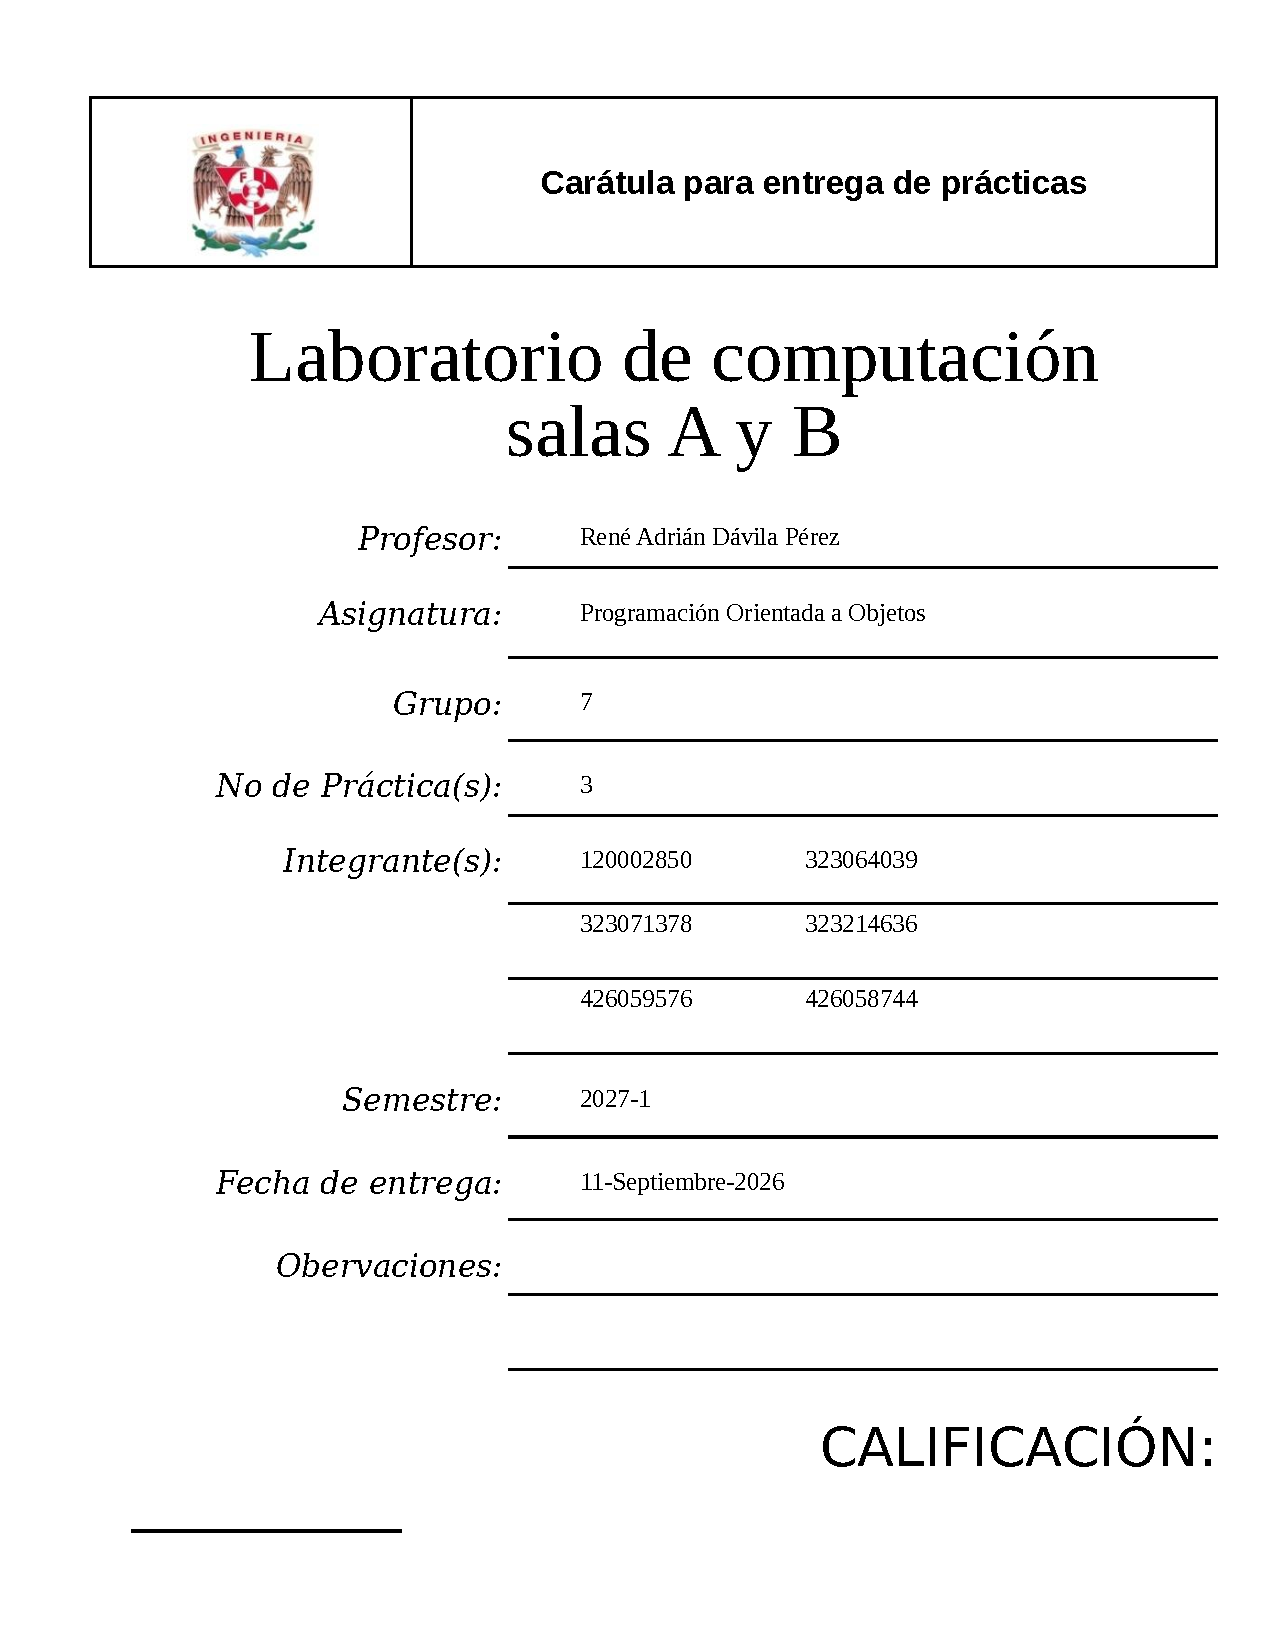
\includepdf[pages=1,pagecommand={}]{caratula.pdf}

\tableofcontents
\clearpage

\section{Introducci\'on}

\subsection{Planteamiento del problema}
La pr\'actica solicita resolver dos necesidades relacionadas con la programaci\'on orientada a objetos. La primera consiste en plantear una interfaz gr\'afica elemental para capturar un usuario y una contrase\~na. La segunda requiere representar tres entidades distintas —un edificio, un autom\'ovil y una bicicleta— mediante clases que implementen una misma interfaz llamada \texttt{HuellaCarbono}. Cada objeto debe calcular su huella con los datos propios de su dominio y la clase principal debe recorrer una lista de referencias comunes para demostrar polimorfismo.

\subsection{Motivaci\'on}
El ejercicio permite observar que una interfaz define un contrato sin obligar a que todas las clases compartan la misma f\'ormula. El edificio relaciona consumo el\'ectrico y factor de emisi\'on; el autom\'ovil relaciona distancia, rendimiento y combustible; la bicicleta expresa que su operaci\'on no produce emisiones directas en el modelo did\'actico. La GUI complementa el aprendizaje al mostrar una interacci\'on visual sencilla con componentes de Swing y un campo especializado para contrase\~nas.

\subsection{Objetivos}
El objetivo general es implementar y comprobar una soluci\'on b\'asica en Java que use una interfaz, implementaciones concretas y polimorfismo. Como objetivos espec\'ificos se establecen: crear las clases \texttt{Edificio}, \texttt{Auto} y \texttt{Bicicleta}; declarar el m\'etodo \texttt{getHuellaCarbono()}; almacenar las instancias en un \texttt{ArrayList<HuellaCarbono>}; presentar una ventana de login con usuario y contrase\~na; documentar cada clase; y comparar c\'alculos esperados con salidas observadas en ejecuci\'on.

\section{Marco Te\'orico}

Una interfaz en Java declara un contrato de operaciones que una clase concreta debe cumplir. La especificaci\'on del lenguaje describe que una clase puede implementar una o varias interfaces y que una referencia al tipo de la interfaz puede utilizarse para invocar operaciones definidas por ese contrato \cite{jls}. En esta pr\'actica, \texttt{HuellaCarbono} solo declara \texttt{getHuellaCarbono()}, mientras que cada clase determina la forma de obtener el valor. La selecci\'on de la implementaci\'on ocurre durante la ejecuci\'on, lo que constituye el polimorfismo utilizado por el recorrido de la lista.

\Needspace{8\baselineskip}
El encapsulamiento concentra los datos de cada entidad dentro de la clase que conoce su significado. Por ello, los consumos, distancias y factores se mantienen como atributos privados, mientras que los m\'etodos p\'ublicos ofrecen consultas y el c\'alculo requerido. La soluci\'on evita herencia porque las tres entidades no forman una jerarqu\'ia natural: comparten el contrato de huella, pero no una estructura de estado com\'un.

La interfaz gr\'afica se construye con Swing. Un \texttt{JFrame} funciona como ventana; \texttt{JTextField} captura el usuario; \texttt{JPasswordField} proporciona un componente apropiado para una contrase\~na; \texttt{JButton} inicia la acci\'on; y \texttt{JLabel} comunica el resultado. La documentaci\'on de Oracle presenta estos componentes como parte de la biblioteca de interfaces gr\'aficas de Java y recomienda asociar acciones a los controles mediante listeners \cite{swing}.

La huella de carbono depende del alcance y de los factores seleccionados. Los inventarios oficiales separan fuentes y unidades, por lo que un factor el\'ectrico debe interpretarse seg\'un la regi\'on y el periodo analizado \cite{epaelectric}. Para mantener el ejercicio reproducible se emplean dos factores did\'acticos expl\'icitos: $0.40\ \mathrm{kg\ CO_2e/kWh}$ para electricidad y $2.31\ \mathrm{kg\ CO_2e/L}$ para gasolina. No se presentan como valores universales; solo permiten comprobar una transformaci\'on aritm\'etica estable. El factor de gasolina se redondea a partir de factores de combusti\'on publicados para inventarios de gases de efecto invernadero \cite{epafactors}.

\clearpage
\section{Desarrollo}

\subsection{Investigaci\'on y an\'alisis de la consulta}
La consulta com\'un se redact\'o para solicitar una explicaci\'on de 90 a 120 palabras sobre dos temas del enunciado: una GUI de login con Swing y el dise\~no de la interfaz \texttt{HuellaCarbono}. El archivo \texttt{doc/Capturas/query.txt} contiene 104 palabras y conserva los ejemplos num\'ericos usados en la implementaci\'on. No se recibieron las seis respuestas originales ni sus im\'agenes; por ello, el reporte incluye una s\'intesis t\'ecnica propia y reserva honestamente los seis espacios de evidencia sin atribuir respuestas a personas concretas.

\Needspace{15\baselineskip}
La primera reserva corresponde a Alan, cuyo avatar de referencia es CJ de GTA y cuyo color de guion es \texttt{\#166A8F}.
\figura{../Capturas/1.png}{Reserva de investigaci\'on 1: Alan; no se aport\'o captura original.}{fig:invalan}

\Needspace{15\baselineskip}
La segunda reserva corresponde a Zo\'e, identificada en la tabla operativa por Snoopy, llamado Snoppy por el equipo, y el color \texttt{\#A52F64}.
\figura{../Capturas/2.png}{Reserva de investigaci\'on 2: Zo\'e; no se aport\'o captura original.}{fig:invzoe}

\Needspace{15\baselineskip}
La tercera reserva corresponde a Luis, con Rabbit como avatar y el color \texttt{\#9A4C16}; no se a\~nade una franquicia no proporcionada.
\figura{../Capturas/3.png}{Reserva de investigaci\'on 3: Luis; no se aport\'o captura original.}{fig:invluis}

\Needspace{15\baselineskip}
La cuarta reserva corresponde a Joseph, con Rick Sanchez como avatar y el color \texttt{\#197349}.
\figura{../Capturas/4.png}{Reserva de investigaci\'on 4: Joseph; no se aport\'o captura original.}{fig:invjoseph}

\Needspace{15\baselineskip}
La quinta reserva corresponde a Hanniel, con el cubo de Geometry Dash como avatar y el color \texttt{\#5941A9}.
\figura{../Capturas/5.png}{Reserva de investigaci\'on 5: Hanniel; no se aport\'o captura original.}{fig:invhanniel}

\Needspace{15\baselineskip}
La sexta reserva corresponde a Alex, con Phineas de Phineas y Ferb como avatar y el color \texttt{\#67531C}.
\figura{../Capturas/6.png}{Reserva de investigaci\'on 6: Alex; no se aport\'o captura original.}{fig:invalex}

\FloatBarrier
\clearpage

\subsection{Interfaz gr\'afica de login}
La clase \texttt{LoginGUI} extiende \texttt{JFrame} e implementa \texttt{ActionListener}. Su formulario contiene un campo de usuario, un campo de contrase\~na, un bot\'on y una etiqueta de estado. La validaci\'on es deliberadamente peque\~na y demostrativa: compara con el usuario \texttt{usuario} y la contrase\~na \texttt{poo8}. Esta decisi\'on permite evidenciar el flujo de entrada, validaci\'on y respuesta sin convertir el ejercicio en un sistema de autenticaci\'on real.

\figura{../Diagramas/LoginGUI_uml.png}{Diagrama UML de la clase LoginGUI.}{fig:loginuml}
\figura{../Diagramas/LoginGUI_flujo.png}{Flujo de captura y validaci\'on del login.}{fig:loginflujo}

\clearpage

\subsection{Contrato de huella de carbono}
La interfaz \texttt{HuellaCarbono} contiene un solo m\'etodo: \texttt{double getHuellaCarbono()}. Al mantener el contrato m\'inimo, el programa principal puede trabajar con referencias del tipo de la interfaz sin preguntar qu\'e clase concreta calcula el valor. El diagrama UML conserva el compartimento de atributos vac\'io porque la interfaz no declara estado, y el flujo representa la delegaci\'on hacia la clase concreta.

\figura{../Diagramas/HuellaCarbono_uml.png}{Diagrama UML de la interfaz HuellaCarbono.}{fig:huellauml}
\figura{../Diagramas/HuellaCarbono_flujo.png}{Flujo conceptual de la operaci\'on getHuellaCarbono.}{fig:huellaflujo}

\clearpage

\subsection{Clase Edificio}
\texttt{Edificio} identifica una construcci\'on por su nombre, consumo anual de electricidad y factor de emisi\'on. La f\'ormula implementada es $H = C \times F$, donde $C$ se mide en kilowatt-hora y $F$ en kilogramos de CO$_2$e por kilowatt-hora. El comportamiento es exclusivo de esta clase porque las otras entidades no utilizan un consumo el\'ectrico anual.

\figura{../Diagramas/Edificio_uml.png}{Diagrama UML de la clase Edificio.}{fig:edificiouml}
\figura{../Diagramas/Edificio_flujo.png}{Flujo del c\'alculo de huella de Edificio.}{fig:edificioflujo}

\clearpage

\subsection{Clase Auto}
\texttt{Auto} identifica un modelo y calcula el combustible utilizado con $L = (K \times R)/100$, donde $K$ es la distancia en kil\'ometros y $R$ es el rendimiento expresado en litros por cada cien kil\'ometros. Despu\'es obtiene la huella con $H = L \times F_g$, usando el factor de gasolina $F_g$. La separaci\'on en dos operaciones hace visible la conversi\'on intermedia y facilita comprobar el resultado.

\figura{../Diagramas/Auto_uml.png}{Diagrama UML de la clase Auto.}{fig:autouml}
\figura{../Diagramas/Auto_flujo.png}{Flujo del c\'alculo de huella de Auto.}{fig:autoflujo}

\clearpage

\subsection{Clase Bicicleta}
\texttt{Bicicleta} conserva un tipo y una distancia recorrida. El alcance del modelo se limita a emisiones operativas directas; por ello, el factor se fija en cero y la f\'ormula $H = K \times 0$ devuelve cero. No se afirma que la fabricaci\'on, alimentaci\'on, mantenimiento o transporte sean nulos, porque esos aspectos no forman parte del enunciado ni del c\'alculo implementado.

\figura{../Diagramas/Bicicleta_uml.png}{Diagrama UML de la clase Bicicleta.}{fig:bicicletouml}
\figura{../Diagramas/Bicicleta_flujo.png}{Flujo del c\'alculo de huella operativa de Bicicleta.}{fig:bicicletaflujo}

\clearpage

\subsection{Clase principal y polimorfismo}
La clase \texttt{Main} crea las tres instancias exigidas y agrega tambi\'en un edificio con consumo cero como frontera pertinente. Las cuatro referencias se guardan en un \texttt{ArrayList<HuellaCarbono>}. El ciclo solo conoce el contrato de la interfaz: imprime la identificaci\'on del objeto y llama a \texttt{getHuellaCarbono()}. El despacho polim\'orfico selecciona la f\'ormula de \texttt{Edificio}, \texttt{Auto} o \texttt{Bicicleta} sin condicionales por tipo.

\figura{../Diagramas/Main_uml.png}{Diagrama UML de la clase principal Main.}{fig:mainuml}
\figura{../Diagramas/Main_flujo.png}{Flujo de creaci\'on, recorrido e invocaci\'on polim\'orfica.}{fig:mainflujo}

\clearpage
\section{Resultados}

\subsection{Casos y resultados num\'ericos}
Los resultados esperados se calcularon antes de ejecutar el programa con las f\'ormulas descritas en el desarrollo. El edificio principal usa $2400 \times 0.40 = 960.00$ kg CO$_2$e. El autom\'ovil usa $480 \times 7/100 = 33.60$ litros y despu\'es $33.60 \times 2.31 = 77.62$ kg CO$_2$e, redondeado a dos decimales. La bicicleta produce cero emisiones operativas directas en el modelo. Finalmente, el edificio frontera permite comprobar que un consumo nulo no introduce una huella espuria.

\begin{table}[!htbp]
\centering
\caption{Comparaci\'on entre el esperado calculado y el observado ejecutado.}
\label{tab:resultados}
\begin{adjustbox}{max width=\textwidth}
\begin{tabular}{p{0.23\textwidth}p{0.29\textwidth}rrp{0.18\textwidth}}
\toprule
\textbf{Objeto} & \textbf{Entrada principal} & \textbf{Esperado} & \textbf{Observado} & \textbf{Estado} \\
\midrule
Edificio Escuela & $2400$ kWh, factor $0.40$ & $960.00$ & $960.00$ & Exitoso \\
Auto Sed\'an & $480$ km, $7.0$ L/100 km, factor $2.31$ & $77.62$ & $77.62$ & Exitoso \\
Bicicleta urbana & $12$ km, factor operativo $0.00$ & $0.00$ & $0.00$ & Exitoso \\
Edificio frontera & $0$ kWh, factor $0.40$ & $0.00$ & $0.00$ & Exitoso \\
\bottomrule
\end{tabular}
\end{adjustbox}
\end{table}

La ejecuci\'on observada tambi\'en confirma la identificaci\'on de cada instancia y el recorrido de la lista mediante la interfaz. No se compar\'o contra una salida inventada: las cifras anteriores se obtuvieron de la salida real de la clase compilada y del JAR, cuyos registros visuales se incluyen en las figuras siguientes.

\figura{../Capturas/compilacion_javac.png}{Compilaci\'on limpia de las seis fuentes Java hacia la carpeta test.}{fig:compilacion}
\figura{../Capturas/empaquetado_jar.png}{Creaci\'on y contenido del \texttt{Practica8.jar}.}{fig:jarcontenido}

\clearpage

\subsection{Ejecuci\'on desde clases y desde JAR}
La clase principal se ejecut\'o directamente desde la carpeta de compilados y posteriormente desde el archivo JAR con manifiesto de entrada. Ambas modalidades produjeron las mismas cuatro huellas: $960.00$, $77.62$, $0.00$ y $0.00$ kg CO$_2$e. El JAR contiene \texttt{Main.class}, la interfaz, las tres implementaciones de huella y la clase de GUI, por lo que no incorpora clases de pr\'acticas anteriores.

\figura{../Capturas/ejecucion_classpath.png}{Salida observada al ejecutar Main desde la carpeta de compilados.}{fig:ejecucioncp}
\figura{../Capturas/ejecucion_jar.png}{Salida observada al ejecutar el trabajo completo desde el JAR.}{fig:ejecucionjar}

La compilaci\'on de \texttt{LoginGUI} fue exitosa y la documentaci\'on se gener\'o de forma independiente. No se declara una ejecuci\'on visual observada de la ventana porque el entorno de trabajo no dispone de un servidor gr\'afico; la verificaci\'on disponible para este componente es compilaci\'on, firmas, Javadoc y revisi\'on est\'atica del flujo. Esta limitaci\'on no afecta la ejecuci\'on determinista de la parte de consola.

\Needspace{9\baselineskip}
\subsection{Documentaci\'on y empaquetado}
Se gener\'o una salida independiente de Javadoc para \texttt{HuellaCarbono}, \texttt{Edificio}, \texttt{Auto}, \texttt{Bicicleta}, \texttt{Main} y \texttt{LoginGUI}, cada una en su directorio bajo \texttt{doc/Javadoc}. Las invocaciones usaron la fuente expl\'icita de una sola clase, visibilidad privada, codificaci\'on UTF-8, classpath de compilados y un sourcepath temporal vac\'io. Tambi\'en se verific\'o que \texttt{test/} contiene solo los compilados finales y que \texttt{lib/} contiene un solo archivo JAR del trabajo.

\clearpage
\section{Conclusiones}

La interfaz \texttt{HuellaCarbono} permiti\'o unificar tres comportamientos que no comparten una jerarqu\'ia de datos. Cada clase conserva sus atributos y su f\'ormula, mientras que \texttt{Main} utiliza una referencia com\'un y una lista homog\'enea. Esta separaci\'on muestra una aplicaci\'on concreta del polimorfismo: el c\'odigo que recorre la colecci\'on no necesita conocer la clase exacta de cada elemento.

Los resultados num\'ericos coincidieron con los esperados calculados antes de ejecutar. La frontera de consumo cero confirm\'o el comportamiento m\'inimo del modelo, y las ejecuciones desde classpath y JAR conservaron la misma salida. Los factores de emisi\'on se mantuvieron como supuestos did\'acticos expl\'icitos, porque una evaluaci\'on real tendr\'ia que seleccionar factores apropiados para una regi\'on, periodo y alcance definidos.

La GUI de login complet\'o el flujo acad\'emico de captura, validaci\'on y respuesta mediante componentes b\'asicos de Swing. Su validaci\'on no pretende sustituir autenticaci\'on segura; su funci\'on es demostrar la interacci\'on gr\'afica solicitada. En conjunto, la pr\'actica relaciona contrato, implementaciones concretas, documentaci\'on y empaquetado reproducible sin agregar una arquitectura innecesaria.

\clearpage
\renewcommand{\refname}{Bibliograf\'ia}
\begin{thebibliography}{99}

\bibitem{jls}
Oracle, \emph{The Java Language Specification, Java SE 25 Edition: Interfaces}, Oracle Corporation, 2025.

\bibitem{swing}
Oracle, \emph{Creating a GUI With Swing}, The Java Tutorials, Oracle Corporation.

\bibitem{epaelectric}
U.S. Environmental Protection Agency, \emph{Emissions \& Generation Resource Integrated Database (eGRID)}, EPA, 2024.

\bibitem{epafactors}
U.S. Environmental Protection Agency, \emph{Emission Factors for Greenhouse Gas Inventories}, EPA, 2024.

\end{thebibliography}

\end{document}
